
%
% File coling2016.tex
%
% Contact: mutiyama@nict.go.jp
%%
%% Based on the style files for COLING-2014, which were, in turn,
%% Based on the style files for ACL-2014, which were, in turn,
%% Based on the style files for ACL-2013, which were, in turn,
%% Based on the style files for ACL-2012, which were, in turn,
%% based on the style files for ACL-2011, which were, in turn, 
%% based on the style files for ACL-2010, which were, in turn, 
%% based on the style files for ACL-IJCNLP-2009, which were, in turn,
%% based on the style files for EACL-2009 and IJCNLP-2008...

%% Based on the style files for EACL 2006 by 
%%e.agirre@ehu.es or Sergi.Balari@uab.es
%% and that of ACL 08 by Joakim Nivre and Noah Smith

\documentclass[11pt, a4paper]{article}
\usepackage{coling2016}
\usepackage{times}
\usepackage{url}
\usepackage{latexsym}
\usepackage{graphicx}
\usepackage{amsmath,amsfonts,amstext,amssymb,amsbsy,amsopn,amsthm,eucal}


%\setlength\titlebox{5cm}

% You can expand the titlebox if you need extra space
% to show all the authors. Please do not make the titlebox
% smaller than 5cm (the original size); we will check this
% in the camera-ready version and ask you to change it back.


\title{Optimization of the Modeling Approach for Predicting the Tolerance Level of Religious Discourse}

\author{Nicolas Venuti \\
  Data Science Institute \\
  University of Virginia \\
  Charlottesville, VA USA \\
  {nmv7de@virginia.edu} \\\And
  Hope McIntyre \\
  Data Science Institute \\
  University of Virginia \\
  Charlottesville, VA USA \\
  {hm7zg@virginia.edu}\\\And
  Donald E. Brown \\
  Data Science Institute \\
  University of Virginia \\
  Charlottesville, VA USA \\
  {brown@virginia.edu} \\}

\date{}

\begin{document}
\maketitle
\begin{abstract}
Religious violence is an important and complicated problem faced by many regions of the world today. The number of incidents has increased in recent years. To combat this problem requires scalable and accurate systems that can predict which groups are likely to engage in violence.
Creating such systems is difficult because of factors such as lingual and cultural differences. These differences limit understanding of group tolerance or tendencies to violence. Recent work has provided a promising new approach to address this challenge by analyzing the performative character of discourse (how words are used) rather than using the semantic or emotive character of text (what the words mean or imply). Results in this paper build on this performative approach.  These results derive from signal processing approaches for extracting word usage features from religious text to efficiently and effectively assess a group's tolerance or predilection to offensive behavior. In addition to improvements to  signal processing algorithms  for performative analysis the paper also describes hyperparameter optimization that can increase the accuracy in estimation of semantic density as well as the predictive accuracy of the lingual flexibility in group discourse. Taken together these results provide a foundation for future work to connect language to group behavior.  

\end{abstract}

\section{Introduction}\label{Intro}

\blfootnote{
    %
    % 
    %
    \hspace{-0.65cm}  
    This work is licenced under a Creative Commons 
     Attribution 4.0 International License.
     License details:
     \url{http://creativecommons.org/licenses/by/4.0/}
    %
    
}

Religious violence has long been one of the most destructive and divisive acts impacting society and, unfortunately, the loss of life and damage associated with these acts has been rising in recent years. In 2014 alone, 12,737 deaths were attributed to just two  radical religious groups: Boko Haram and the Islamic State of Iraq and the Levant (ISIL) \cite{Searcey2015}. Combating this problem requires scalable and accurate systems to predict which groups are likely to engage in violence. 

Most approaches to predicting violent proclivity in groups use the literal or emotive attributes of keywords distributed by the semantic characteristics of these words. New work by  the Global Covenant of Religions Ethnolinguistics Research Team (GCR-ERT) has found that the performative character of discourse, the capacity for language to encapsulate an action or identity, is correlated to the level of intolerance within that discourse. To quantify the performative character of discourse, the GCR-ERT have developed a 1 - 9 language rigidity scale that is used to classify texts as either rigid (scored a 1) or elastic (scored a 9). These rankings are assigned manually by analyzing a wide array of characteristics within religious discourse.  Their work has shown that certain characteristics of discourse, such as the frequency of judgments and the rigidity of keyword contexts, can inform this quantification. 

This paper describes computational methods to uncover and exploit the performative characteristics of religious discourse highlighted by the GCR-ERT in tandem with traditonal semantic signals.  The results here build on earlier work in developing algorithms for performative analysis by implementing more efficient algorithms for text analysis,  improving hyperparameter estimation and enlarging the number and variety of religious texts analyzed. Taken together the contributions in this paper provide a foundation for automated systems to uncover signals of tolerance or violence from the performative characteristics of religious language. The next section provides background on related research. Section~\ref{data} gives an overview of the data used in the analysis, Section~\ref{signals} describes the signals acquired by the performative approach, and Section~\ref{optimization} has the details on the methods for hyperparameter optimization. Finally, Section~\ref{results} shows the results from this work and Section~\ref{conclusions} gives conclusions and future directions.  

\section{Related Work}\label{relatedwork}

Because religious violence is a far-reaching and complex problem, many resources are dedicated to studying the actions and words of groups identified as high-risk. Linguistic approaches to this problem have focused primarily on semantics to classify the goals and intentions of groups (e.g., \cite{brett2005}). While the terms used by groups do correlate with future behaviors, the specific terms may be coded in ways that are difficult for outsiders to understand and interpret \cite{hassner2009}. Often these methods are focused on predicting specific incidences of violence ~\cite{Yang2010}.

Another thread of research has focused on word usage or the performative characteristics in religious language as signaling intentions. Early work by  \newcite{Barsalou1993} showed that shifts in definitions correlate with the representational flexibility of a concept. Later work by \newcite{Sagi2009} has found that a �diversity of contexts� directly correlates with the performative characteristics of words. Their results have influenced this work and Section~\ref{signals} describes the use of their dimensionality reduction threshold.

At a more detailed level, \newcite{Bullinaria2012} evaluated the impact of stop-lists, word stemming, and singular value decomposition (SVD) on the performance of word-word co-occurrence statistics by comparing performance with several generic semantic tasks. They determined that neither word stop-lists nor word stemming significantly impacted performance, minimal context window size gave the best performance, and dimensionality reduction through SVD can improve performance.  

\newcite{Boussidan2011} used a graph built from subsetted co-occurrence tables to create a map of lexical usages of words. Finding the cliques in this graph has interesting results but the computational complexity of computing cliques limits the scalability of this method. \newcite{Cook2010} used a similar approach to detect `amelioration' (a word losing a negative meaning) and `pejoration.' 

Very recent work by \newcite{venuti2016} showed initial results that the pejorative characteristics of language can signal the tolerance level of religious discourse. They developed a judgment identifier along with multiple semantic density algorithms to replicate the frequency of judgments and the rigidity of keyword contexts. Testing showed that performative characteristics of language yield better predictive signals than than semantic-based approaches. This paper builds on and extends that work through more efficient implementations of text analysis algorithms (Section~\ref{signals}), hyperparameter optimization (Section~\ref{optimization}), and a larger, more expansive set of religious texts for testing (Section~\ref{data}).  

\section{Data}\label{data}

The data used to perform this analysis come from online repositories that contained texts from different religious groups with a wide variety of affiliations and language rigidities, as described in Table \ref{table:data}. We collected these texts from their respective online repositories using BeautifulSoup in Python and converted them to .txt files ~\cite{Richardson2015}. Members of the GCR-ERT manually reviewed and annotated the overall document sets with a language flexibility ranking to serve as ground truth for the analysis.

\begin{table}[ht]
\caption{Data Sources}
\begin{center}
\begin{tabular}{lccc}
 \\  \hline
Group & Rank & Affiliation & Number of Doc.  \\ \hline
Westboro Baptist Church 		& 1 & Baptist		& 419 \\
Faithful Word Baptist Church	& 2 & Baptist		& 228 \\
Nouman Ali Khan			& 3 & Sunni Muslim	& 88 \\
Dorothy Day				& 4 & Catholic		& 774 \\
John Piper				& 4 & Baptist		& 579 \\
Steve Shepherd			& 4 & Christian		& 728 \\
Rabbinic texts				& 6 & Jewish		& 166 \\
Unitarian texts				& 7 & Unitarian		& 276 \\ 
Meher Baba				& 8 & Spiritualist	& 265 \\	

\end{tabular}
\end{center}
\label{table:data}
\end{table}

To balance the requirements for increased observations for modeling and the text size requirements for the semantic density algorithms, we randomly placed the documents into bins of 10 for each group. If any individual bin was smaller than half the targeted bin size (i.e., 5 documents), we discarded it so as to not introduce significant sample size disparities. For each group the bins were split into a training set containing 70\% of the bins and a testing set containing the remaining 30\%. 

We normalized and cleaned all the documents prior to signal development to ensure data continuity between each algorithm. We extracted the raw text for each bin, tokenized,  and normalized the text by removing punctuation, converting to lowercase, and converting all numbers to a single symbol. The tokens were stemmed, but stopwords were not removed. These tokens served as the inputs for all signals with the exception of the judgement algorithm.

To identify keywords for the analysis, we applied the Maxent POS Tagger from the python nltk package to the corpus \cite{loper2002}. Word counts were generated for each unique word/POS tag combination for each bin. The top 10 most frequent adjectives and adverbs were selected for each bin and used to as the keywords. These keywords were then fed into the context vector (Subsection \ref{subsect:contextvectors}) and network quantification (Subsection \ref{subsect:network}). 

\section{Signals}\label{signals}

Building on the work in \newcite{venuti2016} we constructed four signals as input to the ranking model; context vectors similarity, judgement fractions, document sentiment, and network quantification. Significant modifications were made to the judgement and sentiment algorithms to better model the requisite features and to provide more normalized outputs. These methods were also reimplemented to reduce computation times and add greater modeling flexibility. The algorithms for the computation of each signal as implemented in this study are described in the following subsections.

\subsection{Sentiment}

We created four sentiment metrics for each group of documents: average percent positive words per document, average percent negative words per document, percent positive documents, and percent negative documents. The sentiment was calculated using a lexicon-based approach. A dictionary of approximately 6,800 positive and negative words, developed by \newcite{Liu2013}, was used. These words were stemmed to ensure maximal matching between the sentiment word list and the pre-processed text. The average percent positive words was calculated as was the percent word matches for each document in the bin. The same procedure was followed for negative words. 

The sentiment of each document was determined by the greater value of word matches (positive or negative). The percent positive documents was created by summing the number of documents with a positive sentiment and dividing by the total number of documents in the bin. The same was done for percent negative documents.

\subsection{Judgment Numbers}\label{subsec:judgment}

To quantify the judgments signal, the CLDS team utilized a custom algorithm in conjunction with a Maxent POS tagger to identify judgments in text through syntactic parsing ~\cite{Hornik2011}. The output of the algorithm is the average proportion of sentences that act as judgments, along with the average number of judgments in each document. The algorithm split each document into sentence segments and word tokens. POS tagging was used on the word tokens to enable the identification of nouns, adjectives, and adverbs. Our algorithm used the POS tagging results to flag a combination of a noun, `to be' verb, and adjective or adverb, the core components of a judgment, in a sentence. The three components were required to be located in that order to be considered a match, which is an added constraint from the previous analysis.  

The number of flagged sentences divided by the total number of sentences was calculated for each document. This value was averaged for each document in the bin to generate the final judgment percentage signal.

\subsection{Context Vectors}
\label{subsect:contextvectors}

To capture the variations in linguistic flexibility of keywords within religious discourse, we implemented a context vector semantic density algorithm in python based on research by \newcite{Sagi2009}. 

Using the pre-processed tokens as described in the data section above, a co-occurrence matrix, $X = [x_{ij}]$ was constructed with $i,j \in \{1,2,\ldots, v\}$, where $v$ is the size of the vocabulary. The $x_{ij}$ elements of $X$ capture how often each word appeared with other words in the vocabulary. This was done by iterating over each word in the bin and counting the words within a $\pm k$ sized window. The result of this was a vector containing the number of times the other words in the vocabulary occurred within a \textit{k}-sized window of that word.  

Once the co-occurrence matrix, $X$, was constructed, a distributional semantic matrix, $D$, was developed to reduce the computational load. $D$ was obtained from $X$ using truncated SVD. This reduced the column space of $D$ to 50 components. 

Next, context vectors were created from $D$. The context vectors for each keyword in the bin were developed by extracting the words within an \textit{r}-sized window surrounding the target and summing the rows of $D$ for the words within the window.  Specifically, let $w_{ij}$ represent the $j$ occurrence of target $i$. So the context vector for this word, $c_{ij}$, is given by 

\begin{equation}
\label{eq:context}
c_{ij}=\sum_{h \in (w_{ij})_{\pm r}} D_{h}
\end{equation}

\noindent where $D_{h}$ is  row $h$ of $D$ and $(w_{ij})_{\pm r}$ is the window of size $r$ around word, $w_{ij}$. 

To calculate the semantic density for each target bin word, we began with the context vectors. Let $C_{i}$ be the set of context vectors found in equation~\ref{eq:context} for target bin word $i$. We then estimated the average cosine similarity of all the context vectors for that word by randomly sampling 2 context vectors from the set, $C_{i}$ and calculated the cosine similarity between them. This was performed over $n=1000$ iterations. The resulting values were averaged to produce the semantic density, $SD$, for that target word as shown below.

\begin{equation*}
SD(w_{i}) = \frac{1}{n}\sum_{k=1}^{n} \frac{c_{ia_{k}}\cdotp c_{ib_{k}}}{||c_{ia_{k}}||* ||c_{ib_{k}}||}
\end{equation*}

\noindent where $a_{k}$, $b_{k}$ are randomly chosen from $C_{i}$ in iteration $k$. To determine the effect of the hyperparameters on average context vector cosine similarity, and in turn prediction, the co-occurrence window length and the context window length were varied. Section~\ref{optimization} discusses the optimization of these parameters.

\subsection{Network Quantification}
\label{subsect:network}

Utilizing the distributional semantic matrix, $D$, we created a graph to estimate semantic density using the igraph package in python \cite{Csardi2006}. This was done by first creating a $v$-$v$ adjacency matrix by computing the cosine similarity of each row $h$ in $D$. Values in this matrix were converted to 0 or 1 based on if they were above or below the determined network adjacency angle threshold, respectively. This matrix was then used to create a graph where a node represents a word and an edge was assigned between two nodes if the associated value in the adjacency matrix was 1. The choice of threshold is discussed in Section~\ref{optimization}.

This graph was then used to calculate eigenvector centrality. Eigenvector centrality scores the influence of a network on a node by looking at the number of influential nodes to which it is connected \cite{Estrada2005}. This number of connected nodes was used as a proxy for the linguistic flexibility of a word. The more varied the connection the higher number of uses of that word.

\section{Hyperparameter Optimization} \label{optimization}

To improve performance of the approach, key hyperparameters affecting the computation of the linguistic signals were identified and optimized.  Parameter assessment also provides data to guide directions for future research.

\subsection{Co-Occurrence Window}
\label{cooc window}

The first parameter selected for optimization was the co-occurrence window, $k$. This window directly affects the representation of the distribution of the language within the corpus. A larger window will incorporate more information about the words occurring around other words. This may better encapsulate the language or may add noise to the analysis. For this reason, windows of size 2 to 6 were explored during hyperparameter optimization. The ideal value was determined by that which best improved the accuracy of the model over a 3-fold cross validation.

\subsection{Context Window}
\label{sect:context window}

Context Window size, $r$, was also analyzed to determine the optimal value. In contrast to the co-occurrence window which measures general word usage, the context window size impacts the specific measure of a word's usage. Without knowledge of how the proximity of a word affects the analysis of the variability of its usage, we varied the window size from 2 to 6 to determine the window size with the best predictive performance.

\subsection{Network Adjacency Angle}
\label{sect:angle}

Finally, the network adjacency angle threshold was optimized. As discussed in Subsection~\ref{subsect:network} the network adjacency angle threshold was used to assign connections between nodes in a graph.  This threshold can significantly impact the accuracy of estimates of word usage variability. This is due to the fact that an inaccurate value of network adjacency angle could over or under estimate the relationship of words in the graph. To investigate this the threshold value was varied by 15 degree increments over the range of 15 to 75 and the optimal parameter value was determined by that which most improved model performance.

\section{Results}
\label{results}

To evaluate the effects of the hyperparameters on the semantic density and network signals, we conducted a grid search of the co-occurrence window, the context window and the network adjacency angle. By varying these parameters we sought to better understand the effects of these parameters on the linguistic signals and also to understand how these signals map to the linguistic flexibility of the  groups. 

For the random forest regression model Figure \ref{fig:EVC_SD_surface} (a) plots the average semantic density of the groups versus the co-occurrence  and context vector window sizes. By plotting the average semantic density in relation to  co-occurrence window ranges of 2-6 and context window ranges of 2-6, this figure shows that an increase of these window sizes results in an increase of the average semantic density of the keywords, although there are multiple modes. Overall these results have an intuitive explanation. Increasing the window ranges allows for greater information to be held in the context vectors and, in turn, results in a cosine similarity closer to one. This figure also shows that a limit is reached at a co-occurrence window of 5 and a context vector window of 5, where the average semantic density settles just above an average cosine similarity of 0.75. This indicates that little gain can be achieved by increasing these window sizes further, as there would be little distinction in the average semantic density of the keywords in the analysis.

\begin{figure}[!h]
\begin{center}
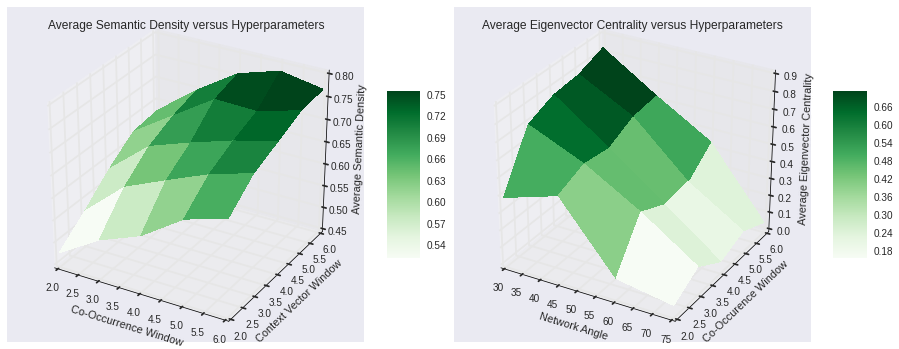
\includegraphics[width = \textwidth]{figs/EVC_SD_surface}
\caption{(a) Average semantic density vs. dependent hyperparameters (b) Average eigenvector centrality vs. dependent hyperparameters}
\label{fig:EVC_SD_surface}
\end{center}
\end{figure}

Figure \ref{fig:EVC_SD_surface} (b) contains the co-occurrence window size and network angle  plotted against the average eigenvector centrality for the SVM regression model.  Although there is distinct mode at a co-occurrence window of 5 and a context vector window of 3, generally the average eigenvector centrality trends upward as the co-occurrence window size increases and the network adjacency angle decreases. These results also have intuitive explanations. An increase in the co-occurrence window size results in a greater connection between the words within the discourse, and the lower adjacency angle produces more edges between the nodes within the graphs. As eigenvector centrality is a bounded variable between 0 and 1, we see that the limit of 1 is nearly reached under the maximal conditions of 30 degrees and a co-occurrence window size of 6. We anticipate that this limit would be achieved by increasing the co-occurrence window or decreasing the network angle further.


To determine the relationship between average semantic density and group rank, the group rank is plotted against the average semantic density of the group, while varying the co-occurrence window and context vector.  This is shown in Figure \ref{fig:multipleAVGSD}.  In this figure the average semantic density is typically higher for groups with a lower rank. The range between the highest semantic density and the lowest semantic density appears to decrease as the co-occurrence window size and the context vector window size increases. The ideal configuration of co-occurrence window size and context vector window size would yield a linear relationship between semantic density and group rank, as that would provide a linear separation boundary for the learning algorithms used. With this in mind a visual inspection of Figure \ref{fig:multipleAVGSD} indicates that a lower configuration may provide this trend, although there is not an explicit separation for any of the configurations.

\begin{figure}[!h]
\begin{center}
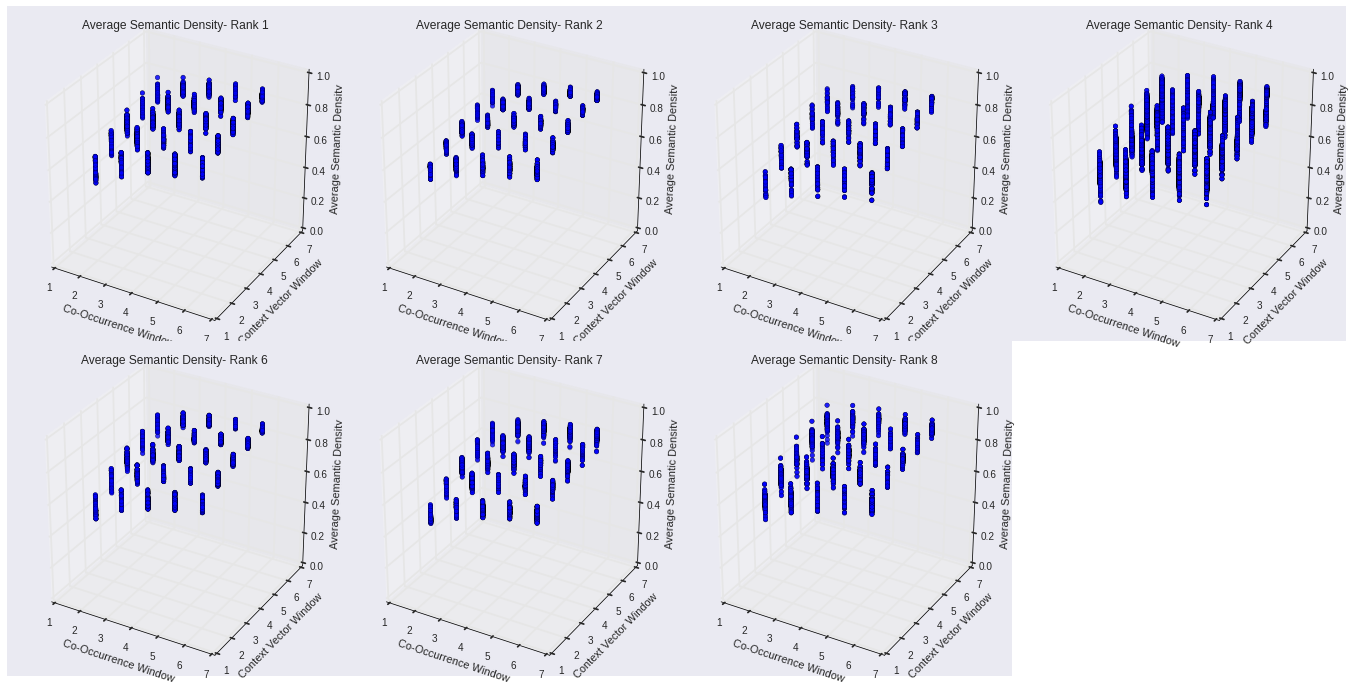
\includegraphics[width = \textwidth]{figs/multipleAVGSD}
\caption{Average Semantic Density versus Hyperparameters}
\label{fig:multipleAVGSD}
\end{center}
\end{figure}

Similar to the analysis above, we also analyzed the distribution of average eigenvector centrality to group rank, as the co-occurrence window and network adjacency angle are varied. From this we found no combination of network angle threshold, co-occurrence window size, and context vector window size within the search space that displays a visually discernible separation or trend between the output eigenvector centrality and the group rank. Hence, none of the configurations produce separable results. As this metric is determined through the selection of keywords, it appears that a different methodology is needed.

With the tandem of performative and semantic based signals we used support vector machine regression (SVM-R) and random forest regression to score the linguistic flexibility of the groups. Both methods can handle the bounded continuous response variable, as well as nonlinear input relations. In \newcite{venuti2016} these methods also outperformed the neural networks.

We calculated model performance given an allowed error margin of 1, as shown in Eq. \ref{eq:acc 1} and Eq. \ref{eq:acc 2}, to account for the natural fluctuations in linguistic flexibility.

\begin{equation}
\label{eq:acc 1}
acc(bin, model) = 
\begin{cases} 
1, & \text{if } |\hat{y}-y| \leq 1 \\
0, & \text{otherwise}
\end{cases}
\end{equation}

\begin{equation}
\label{eq:acc 2}
acc(model) = \frac{1}{|bins|} \sum_{bin  \epsilon  bins} acc(bin, model)
\end{equation}

This accuracy metric was used to evaluate the predictive performance over the range of context vector windows and co-occurrence window for the each model type, random forest and SVM-R, and averaged over the range of network angles.  Figure \ref{fig:RF_SVM_accuracy}(a) shows a tighter range within the lowest performing average accuracy and the highest performing average accuracy. The figure also indicates there are multiple peak accuracies at several parameter combinations,however, the highest concentration appears to be at the lower co-occurrence and context vector window sizes. Conversely, Figure \ref{fig:RF_SVM_accuracy}(b) shows a much larger difference between the lowest performing accuracy and the highest performing accuracy. Furthermore, there is a distinctive trend trend in which there is improved predictive power as the co-occurrence window decreases and the context vector window increases, with optimal levels present at the co-occurrence window size of 2 and the context vector window size of 6.

\begin{figure}[!h]
\begin{center}
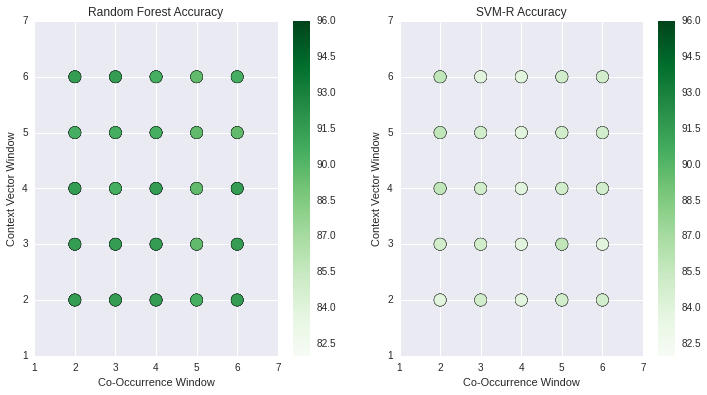
\includegraphics[width = .9\textwidth,keepaspectratio]{figs/RF_SVM_accuracy}
\caption{Model Performance (a) RF (b) SVM}
\label{fig:RF_SVM_accuracy}
\end{center}
\end{figure}


Table \ref{tab:accuracy} shows the increase in accuracy from the  improved implementations of the signal processing algorithms in this paper (Section \ref{signals}) versus the results reported in \newcite{venuti2016}. These results come from three-fold cross-validation. The random forest regression shows the most improvement. These results are important because they provide additional evidence obtained with an enlarged data set that performative-based signals from religious text can predict tolerance. 

\begin{table}[ht]
\caption{Accuracy Comparison for Signal Processing}
\begin{center}
\begin{tabular}{lrr}
\hline
Method & Previous Signal Processing & Improved Signal Processing \\ \hline
SVM- R & 84\% & 86\% \\
RF- R 	& 86\% & 92\% \\ 
\end{tabular}
\end{center}
\label{tab:accuracy}
\end{table}%
 
\section{Conclusions}
\label{conclusions}

As the number of incidents of religious violence continues to increase, the need for scalable and accurate prediction systems intensifies. Analysis of the semantic characteristics of language has shown promise in prior research and the manual evaluation of performative characteristics by the GCR-ERT, has produced good predictions of flexibility of keywords in religious discourse. The work in this paper has significantly extended these previous results and shown the effects hyperparameter selection has on the performative features, and in turn the effects these parameters have on overall prediction accuracy. By visualizing these effects, a more informed methodology can be developed in future studies. 

While these results show promise, additional work is needed. As only a select set of values were tested due to computational demands of higher window sizes, further studies need to be conducted to further understand the effects of hyperparameters on these signals. Additionally, the process around identifying keywords needs to be further analyzed, so more robust group-specific keywords can be identified automatically, which may provide more separable trends in the network quantification and semantic density analyses. Lastly, a wider array of documents needs to be analyzed with a greater variety of religious groups in each class. This would prevent the algorithms from over-fitting based on group specific tendencies and illustrate the performative characteristics of these group's discourse.

\section*{Acknowledgements}

The acknowledgements should go immediately before the references.  Do
not number the acknowledgements section. Do not include this section
when submitting your paper for review.

\newpage
\bibliographystyle{acl}
\bibliography{coling2016}


\end{document}

   
\grid
\grid
\grid
